\documentclass{article}

%%%
% All the document and template configuration is defined in here.
%%%

% General formatting
\usepackage[a4paper, left=3cm, right=3cm, top=2.5cm, bottom=3.5cm]{geometry}
\usepackage[parfill]{parskip}
\usepackage[utf8]{inputenc}
\usepackage[T1]{fontenc}
\usepackage{microtype}
\usepackage{titlesec} % Used to format section headers
\usepackage{setspace} % Used to customize line/paragraph spacing

% Package for custom headers and footers
\usepackage{scrpage2}

% Font settings
\usepackage{fontspec}

% Math-related
\usepackage{amsmath,amssymb,amsfonts,amsthm}

% Bibliography settings
\usepackage[style=ieee,backend=bibtex]{biblatex}

% Enabling internal document links and hyperlinks
\usepackage[hidelinks]{hyperref}

% Language-related
\usepackage{hyphenat}
% \usepackage[ngerman]{babel} % Uncomment if you intend to write in german

% Other
\usepackage{lipsum} % For generating placeholder text
\usepackage{xcolor}
\usepackage{tikz} % For painting stuff!
\usepackage{graphicx}


%%%
% Custom font
%%%

\setmainfont{Segoe UI}

%%%
% Custom headers and footers
%%%

\pagestyle{scrheadings}
\clearscrheadfoot % Clear default headers and footers
\ifoot{\metaauthor}
\cfoot{\translationpage\hspace{2pt}\thepage}
\ofoot{
    \includegraphics[width=1.5cm]{assets/graphics/footer-logo.pdf}
}

%%%
% Changing section header formatting
%%%

\newcommand*\circled[1]{\tikz[baseline=(char.base)]{
    \node[shape=circle,draw=gray!30,text=black,line width=1mm,inner sep=3pt] (char) {#1};}}

\titleformat{\section}{
    \LARGE\filcenter % Formatting
}{\circled{\thesection}}{
    0cm % Distance between section numbering and header text
}{
% Header text prefix
}

\titleformat{\subsection}{
    \Large % Formatting
}{\thesubsection}{
    0.1cm % Distance between section numbering and header text
}{
% Header text prefix
}

\titleformat{\subsubsection}{
    \large % Formatting
}{\thesubsubsection}{
    0.1cm % Distance between section numbering and header text
}{
% Header text prefix
}

%%%
% Custom table of contents
%%%

\makeatletter
\renewcommand{\tableofcontents}[1][\contentsname]{%
    \section*{#1}

    \begin{center}
        \dotfill
    \end{center}

    \onehalfspacing
    \@starttoc{toc}
    \singlespacing

    \begin{center}
        \dotfill \\[1.5cm]
    \end{center}
}
\makeatother


% Define meta-data
\newcommand{\metatitle}{A modern and minimal LaTeX template}
\newcommand{\metaauthor}{Benjamin Eder}
\newcommand{\metaemail}{beder@hm.edu}

% Some translations (adapt for the target language)
\newcommand{\translationpage}{Page}

% Define bibliography file
\addbibresource{refs.bib}

\begin{document}

    %%%
    % TITLE
    %%%
    \begin{center}
        \Huge \metatitle \\[0.6cm]
        \large \metaauthor \hspace{3pt} (\textit{\href{mailto:\metaemail}{\metaemail}}) \\[1.5cm]
    \end{center}

    \tableofcontents % Uncomment if you don't want a table of contents

    \section{Introduction}
\label{sec:introduction}

Example of a citation~\cite{latexcompanion}.

\lipsum[1]

\begin{figure}
    \centering
    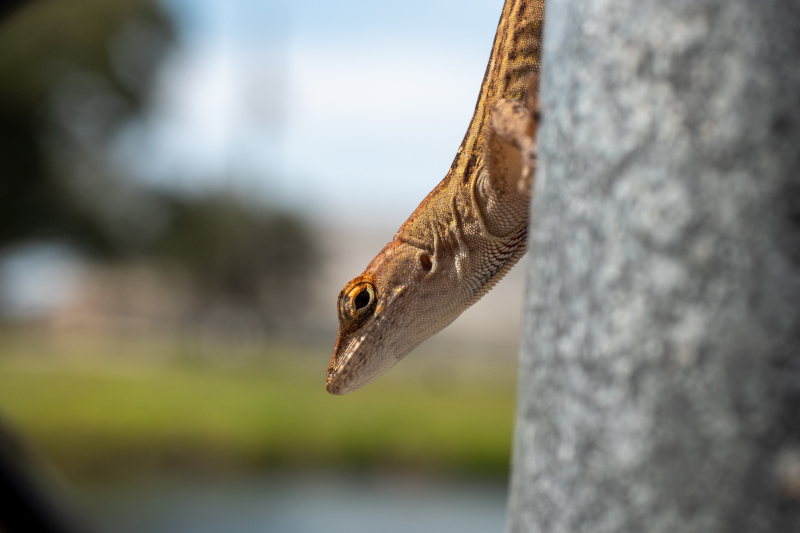
\includegraphics[width=0.8\textwidth]{assets/graphics/example.jpg}
    \caption{A picture I took a while ago!}
    \label{fig:test-figure}
\end{figure}


\section{Methods and tools}
\label{sec:methods-and-tools}

\subsection{Subsection 1}
\label{subsec:subsec1}

\lipsum[1]

\subsection{Subsection 2}
\label{subsec:subsec2}

\lipsum[2]

\subsubsection{Subsubsection 1}
\label{subsubsec:subsubsec-1}

Hello World!
Some math? \(\begin{bmatrix}
                 1 & 2 \\
                 3 & 4
\end{bmatrix}\)

\subsubsection{Subsubsection 2}
\label{subsubsec:subsubsec-2}

\lipsum[6]

\subsection{Subsection 3}
\label{subsec:subsec3}

\lipsum[3]


\section{Results}
\label{sec:results}

\lipsum[2]

\subsection{Subsection 1}
\label{subsec:subsec12}

\lipsum[3-6]

\subsection{Subsection 2}
\label{subsec:subsec13}

\lipsum[7-10]


\section{Discussion}
\label{sec:discussion}

\lipsum[1-2]

\subsection{Subsection 1}
\label{subsec:subsec123}

\lipsum[2-3]

\subsection{Subsection 2}
\label{subsec:subsec134}

\lipsum[11-12]


\section{Summary}
\label{sec:summary}

\lipsum[1-3]


    \printbibliography

\end{document}
